\documentclass{article}
\usepackage[utf8]{inputenc}

\usepackage{graphicx}

\begin{document}
\begin{titlepage}

\newcommand{\capaDisciplina}{Introdução à Computação 2020.2}
\newcommand{\capaProfessor}{Professor: Adriano Lorena Inácio de Oliveira}
\newcommand{\capaAtividade}{Reconhecimento do uso de óculos}
\newcommand{\capaAutores}{João Victor Soares Silva \\ Talita Giovanna Xavier de Oliveira}
\newcommand{\capaData}{24 de Agosto de 2021}

\newcommand{\HRule}{\rule{\linewidth}{0.5mm}}

\center

\textsc{\textbf{\Large \capaDisciplina}}\\[0.2cm]
\textsc{\textbf{\large \capaProfessor}}\\[0.5cm]

%--------------------------------------------------------%
%                         TÍTULO                         %
%--------------------------------------------------------%

\vspace{5.0cm}

\HRule \\ [0.4cm]
{\huge \textbf{\capaAtividade}}\\[0.4cm]
\HRule \\ [1.4cm]

\vspace{3.0cm}
\begin{figure}[ht]
    \centering
    
\includegraphics[scale= 0.2]{Horizontal-Vermelho-Logotipo-CIn-UFPE.png}
    \label{imagem_um}
\end{figure}

\textbf{\large \capaAutores}

\vspace{0.5cm}
\textbf{\capaData}

\end{titlepage}

\section{Do Projeto}
O projeto visa demonstrar a necessidade do uso de óculos de acordo com os dados requisitados pelo programa usado, que serão uma imagem retirada do Google, com o intuito de reconhecer o uso de óculos, e algumas respostas obtidas a partir de uma pequena árvore de decisão.

\section{Dos Dados}
Os dados utilizados na fase de treinamento foram adquiridos do Google Imagens e com intuito de melhorar a taxa de acerto (\textit{accuracy}) foram privilegiadas as imagens frontais (\textit{selfies}). Na label "com óculos" foram depositadas 46 imagens de diferentes pessoas e raças, diferentes ângulos e diferentes tipos de óculos, afim de tornar o aprendizado mais efetivo. Na label "sem óculos" foram depositadas 47 imagens de diferentes pessoas e raças, diferentes ângulos e diferentes tipos de óculos.

\section{Do código}
\par
\begin{figure}[ht]
    \centering
    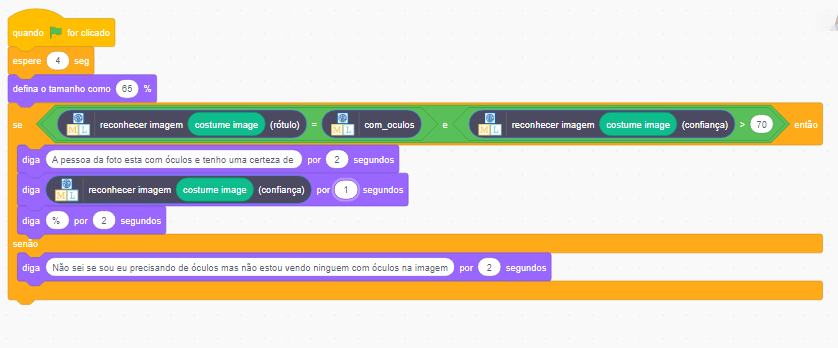
\includegraphics[scale= 0.4]{projeto IC.png}
    \label{imagem_um}
\end{figure}

\section{Dos testes de validação}
Em geral os resultados foram satisfatórios.A plataforma \textit{Machine Learning for Kids} nos permite usar no máximo apenas 100 imagens para o classificador. Sendo um número pequeno quando se compara aos classificadores com milhares de imagens. No entanto, apesar dessa limitação, o programa obteve uma alta taxa de acertos tanto em ambientes escuros quanto em ambientes com iluminação boa em ambiente controlado. Além disso, todos os testes obtiveram uma alta taxa de certeza.

\end{document}
